\newpage
\subsubsection{Energieversorgung}
\begin{figure}[h]
\centering
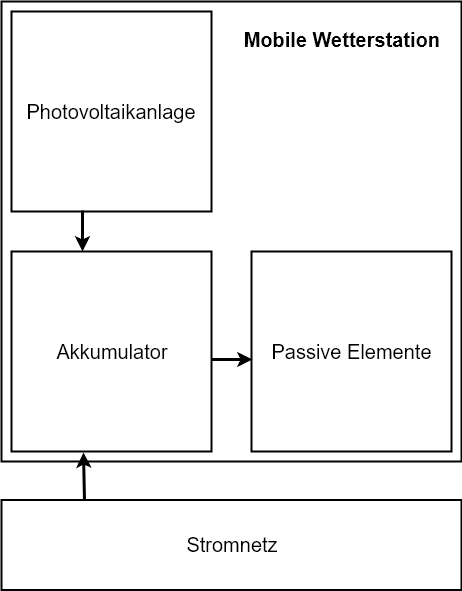
\includegraphics[scale=0.5]{graphics/Konzeptdiagramme/Energieversorgung_1.PNG}
\caption{Energieversorgung des Systems mit Systemgrenze}
\label{fig:Energieversorgung_1}
\end{figure}
In Abbildung \ref{fig:Energieversorgung_1} ist die Systemgrenze der mobilen Wetterstation ersichtlich. Innerhalb der Systemgrenze befinden sich die Photovoltaikanlage, der Akkumulator und die passiven Elemente der mobilen Wetterstation. Ausserhalb der Systemgrenze befindet sich das Stromnetz. Durch die Pfeile wird der Energiefluss aufgezeigt, welcher von der Photovoltaikanlage und vom Stromnetz in den Akkumulator fliesst und von dort aus die passiven Elemente (MCU, Sensorik, RTC, Datenspeicherung, Kommunikationsmodule) der mobilen Wetterstation speist.\\
Der Akku bildet das Kernstück der Energieversorgung, da dieser die Quelle für die mobile Wetterstation ist. Um diesen vor Schäden zu schützen, ist eine Ladeschaltung notwendig, welche eine Überladungs- und Unterladungsschutz beinhaltet. Die Betriebszeit der mobilen Wetterstation hängt im wesentlichen von der Betriebszeit des Akkumulators ab. Um die Betriebszeit des Akkumulators zu verbessern, soll eine Photovoltaikanlage diesen während des Betriebs laden. Ausserdem soll der Akkumulator ebenso mit einem Stecker über das Schweizer Stromnetz ladbar sein. Falls es dennoch zur kompletten Entladung oder zu einem Defekt des Akkumulators kommt, soll dieser im Idealfall leicht austauschbar sein, was als Wunschziel definiert wurde.\\